\documentclass[12pt]{report}
\usepackage{geometry} % see geometry.pdf on how to lay out the page. There's lots.
\geometry{a4paper} % or letter or a5paper or ... etc
\usepackage{graphicx}

% \geometry{landscape} % rotated page geometry

% See the ``Article customise'' template for come common customisations

\title{SSEnext Modular Device Support}
\author{Dave Astels}

%%% BEGIN DOCUMENT
\begin{document}

\maketitle
%\tableofcontents

\chapter{Overview}

One of the key features of the SSEnext architecture is modular device
support. This will allow new devices to be added without having to
modify, rebuild, redownload, or reinstall SSEnext\footnote{In the
  majority of cases. There may be new devices that require changes to
  the core apps.}.

There are three aspects of device support that we need to be concerned
with:
\begin{enumerate}
\item client,
\item database,
\item and device firmware interaction.
\end{enumerate}

Figure~\ref{fig:blockdiagram} shows the relationship between SSEnext
and a device module.

\begin{figure}[htbp] %  figure placement: here, top, bottom, or page
   \centering
   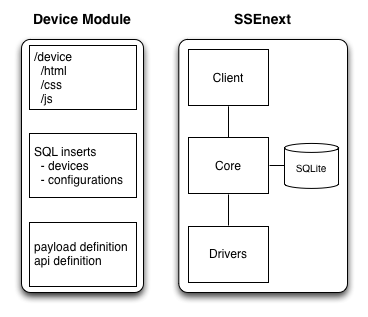
\includegraphics[width=5in]{block_diagram.png} 
\caption{Overview of modular device support.}
\label{fig:blockdiagram}
\end{figure}


This document will explore all three in order.


\chapter{Client}



\chapter{Database}

\section{Device record}

There needs to be a record in the \verb|records| table for each device
supported by the system.

\section{Configuration records}

Depending on the device, SteelSeries may create and include
configurations that are installed as part of the support of that
device. The need to be added to the \verb|configurations| table.



\chapter{Device interaction}



\section{Data definition}

\begin{verbatim}
(def-struct led
     (def-field red uint8)
     (def-field green uint8)
     (def-field blue uint8)
     (def-field mode uint8))

(def-struct cpi
     (def-field unbind uint8)
     (def-field x uint16)
     (def-field y uint16)
     (def-field led led))
\end{verbatim}

These delarations result in the structure shown in Figure~\ref{fig:defstructure} 

\begin{figure}[htbp] %  figure placement: here, top, bottom, or page
   \centering
   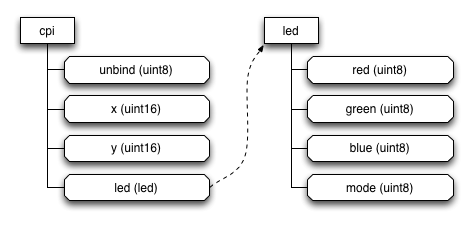
\includegraphics[width=5in]{def_structure.png} 
\caption{Definition structure.}
\label{fig:blockdiagram}
\end{figure}

That structure then gets process, flattening it, tagging each field
with it's path in the original structure, and computing the bytearray
offset of each field (to ensure proper alignment). the result is shown
in Figure~\ref{fig:flattened}.

\begin{figure}[htbp] %  figure placement: here, top, bottom, or page
   \centering
   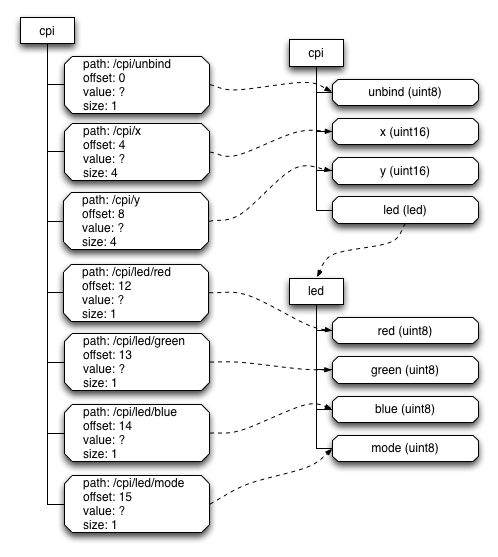
\includegraphics[height=6in]{flat_structure.png} 
\caption{processed structure.}
\label{fig:flattened}
\end{figure}

\begin{figure}[htbp] %  figure placement: here, top, bottom, or page
   \centering
   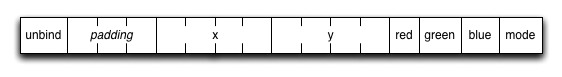
\includegraphics[width=6in]{bytearray.png} 
\caption{processed structure.}
\label{fig:bytearray}
\end{figure}

\begin{verbatim}
{
  "cpi": {
    "unbind": 1,
    "x": 1200,
    "y": 1400,
    "led": {
      "red": 255,
      "green": 255,
      "blue": 100,
      "mode": 2
    }
  }
}
\end{verbatim}


\section{JSON transformations}

\section{API definition}


\end{document}
